% !TEX encoding = UTF-8 Unicode
%!TEX root = main.tex
% !TEX spellcheck = en-US
%%=========================================

%%%%%%%%%%%%%%%%%%%%%%%%%%%%%%%%%%%%%%%%%%%%%%%%%%%%%%%%%%%%%%%%%%%%%%%%%%%%%%%%
\chapter{Performance}
\label{ch:performance}


Benchmarking performance of a concurrency library is not intuitive. Some might even argue performance is not important, but rather the abstractions are correct. However, some metrics of parallel programs can be tested.

For this benchmark, a set of concurrent programs are tested with various degrees of parallelism. Metrics such as concurrent throughput, sequential speed, and load balancing are factors which can influence performance.

To have some appropriately comparable benchmarks, entries from \cref{sec:multicore_csp_existing} are included. occam and XC are however not included, as they require proprietary hardware to run on multicore architectures. C++CSP2 is also not included because of difficulties of implementing benchmark tests which did not result in spurious segmentation faults by the library during execution.

Additionally, singlecore versions of \Proxc{} and Go are included to observe the potential speedup in performance with multicore. \Proxc{} implements a singlecore runtime system with a round robin scheduling policy, while Go implements singlecore runtime system by setting the number of schedulers to one with \texttt{GOMAXPROCS}. C++CSP has no support for a singlecore runtime system, and therefore only the multicore version is included.

All code for the different benchmark tests can be found in \cref{ch:benchmark_code}.


%%%%%%%%%%%%%%%%%%%%%%%%%%%%%%%%%%%%%%%%%%%%%%%%%%%%%%%%%%%%%%%%%%%%%%%%%%%%%%%%
\section{Benchmark Setup}
\label{sec:benchmark_setup}


All benchmarks performed in this chapter are computed on the same machine; a desktop PC with an Intel\textsuperscript{\textregistered} Core\textsuperscript{\texttrademark} i7-4790 4GHz processor with 8 logical cores, 16GiB DDR3 RAM, running Ubuntu\textsuperscript{\textregistered} 16.04 xenial, x86\_64 Linux\textsuperscript{\textregistered} 4.4.0 as operating system.

Intel Core is a registered trademark of Intel Corporation, Linux is the registered trademark of Linus Torvaldsen in the U.S. and other countries, Ubuntu is a registered trademark of Canonical Ltd.


%%%%%%%%%%%%%%%%%%%%%%%%%%%%%%%%%%%%%%%%%%%%%%%%%%%%%%%%%%%%%%%%%%%%%%%%%%%%%%%%
\section{Benchmark Tests}
\label{sec:benchmark_tests}


Three type of benchmark tests are performed: \textit{extended commstime}, \textit{concurrent mandelbrot} and \textit{concurrent prime sieve}. These three tests have various degrees of sequential and parallel characteristics, aiming to highlight the concurrency adaptation capabilities, the concurrent throughput, and how well each entry scales with an increasing amount of parallel work load.


%%%%%%%%%%%%%%%%%%%%%%%%%%%%%%%%%%%%%%%%
\subsection{Extended Commstime}


The extended commstime test is a custom derivation of the original commstime test. The original commstime test \citep{roger2001commstime} is a pseudo\hyp{}standard benchmark for testing sequential channel communication between processes. Three processes called \textit{prefix}, \textit{delta} and \textit{successor} creates a channel cycle, sending an integer in loops. Each loop increments the integer. A fourth process, called \textit{consumer}, receives the integer on each loop cycle. The consumer receives an integer a number of times and calculates the average time to receive the integer. The commstime test mostly gives a metric for the overhead regarding channel communication.

Channel communication overhead is not that interesting of a metric with dynamic multithreading. Commstime is however a good metric for a programs adaptability of sequential programs, as all processes create an sequential dependency. I therefore propose the \textit{extended commstime} test. Instead of three processes in a channel communication cycle, $N$ processes are created in a chain of channel communications, creating a variable sized cycle.

The extended commstime varies the chain length from $N=1$ to $1000$. For each chain length value of $N$, the time to receive $100$ integers divided by the chain length is averaged over $50$ runs. 

The results for the extended commstime test are presented in \cref{fig:extended_commstime}.

\begin{figure}[h!]
    \centering
    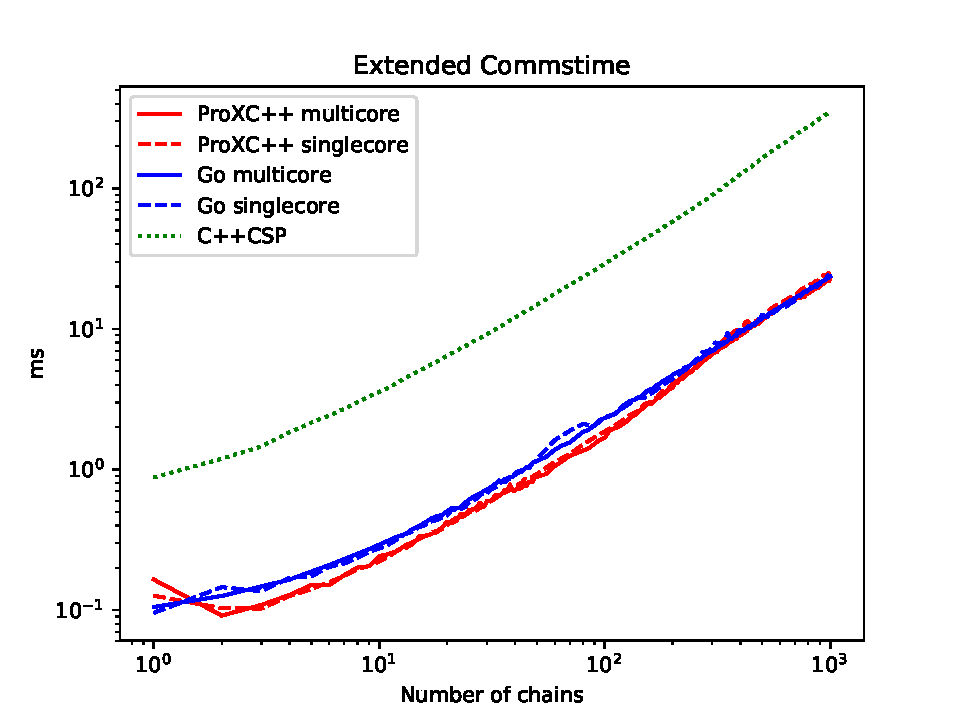
\includegraphics[width=0.9\linewidth]{fig/extended_commstime}
    \caption{Results of extended commstime. The Y axis has a logarithmic scaling.}
    \label{fig:extended_commstime}
\end{figure}


\FloatBarrier
%%%%%%%%%%%%%%%%%%%%%%%%%%%%%%%%%%%%%%%%
\subsection{Concurrent Mandelbrot}
\label{subsec:concurrent_mandelbrot_test}


Some problems are embarrassingly parallel \citep{wilkinson1999parallel}, where little to no effort is needed to separate the work load into parallel tasks. The Mandelbrot set is a perfect example of an embarrassingly parallel problem, where each point in the set can be calculated independently of each other.

Generating a Mandelbrot set is perfect for testing the parallel capabilities of the entries, such as how good the load balancing is.

For this benchmark, the Mandelbrot set is computed in the domain $x\in[-2.1;1.0]$ and $y\in[-1.3;1.3]$ with a resolution of a given dimension $D$. The set is split into $D$ number of lines on the Y axis, where each line consists of $D$ points evenly distributed along the X axis. Each line represents some parallel unit of work.

All lines are computed in a map\hyp{}reduce manner, where some worker processes each calculates a full line at a time. Two approaches will be tested: a hard coded optimal distribution of work, and dynamic sub\hyp{}optimal distribution of work.

Both approaches tests for the same; for a given dimension from $D=1$ to $1000$, how long does it take to calculate all lines, averaged over $100$ rounds. 

The hard coded optimal distribution is implemented by having the number of worker processes equal to the number of logical cores, $8$ in this case. Each worker process receives a line to calculate from a channel, where a producer process is on the other end continuously sending new lines to calculate. A consumer process receives finished calculated lines on a channel from the worker processes.

Note that for the singlecore version, only $1$ worker process is spawned as only a single core is available.

The results for the hard coded Mandelbrot test are presented in \cref{fig:mandelbrot_hardcoded}.

\begin{figure}[h!]
    \centering
    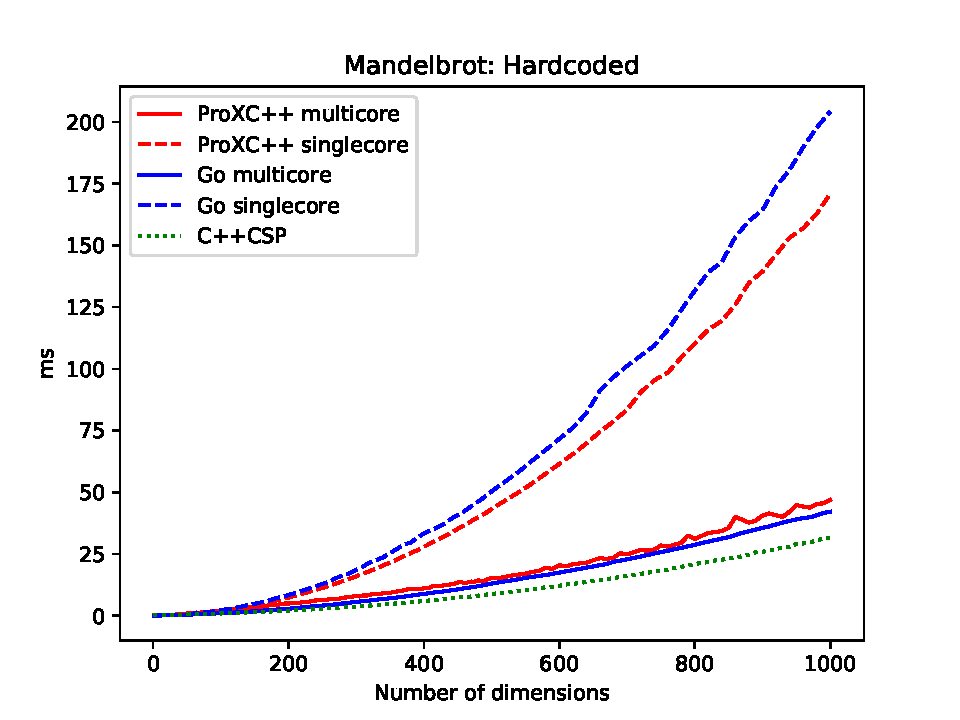
\includegraphics[width=0.9\linewidth]{fig/mandelbrot_hardcoded}
    \caption{Results of concurrent Mandelbrot with hard coded number of workers.}
    \label{fig:mandelbrot_hardcoded}
\end{figure}

The dynamic sub-optimal distribution is implemented by having worker processes each dedicated for calculating a single line, meaning a total of $D$ worker processes will be spawned for a dimension $D$. All worker processes will be spawned simultaneously. At consumer process will receive finished calculated lines on a channel from the worker processes, just as the hard coded Mandelbrot test.

The results for the dynamic Mandelbrot test are presented in \cref{fig:mandelbrot_dynamic}.  

\begin{figure}[h!]
    \centering
    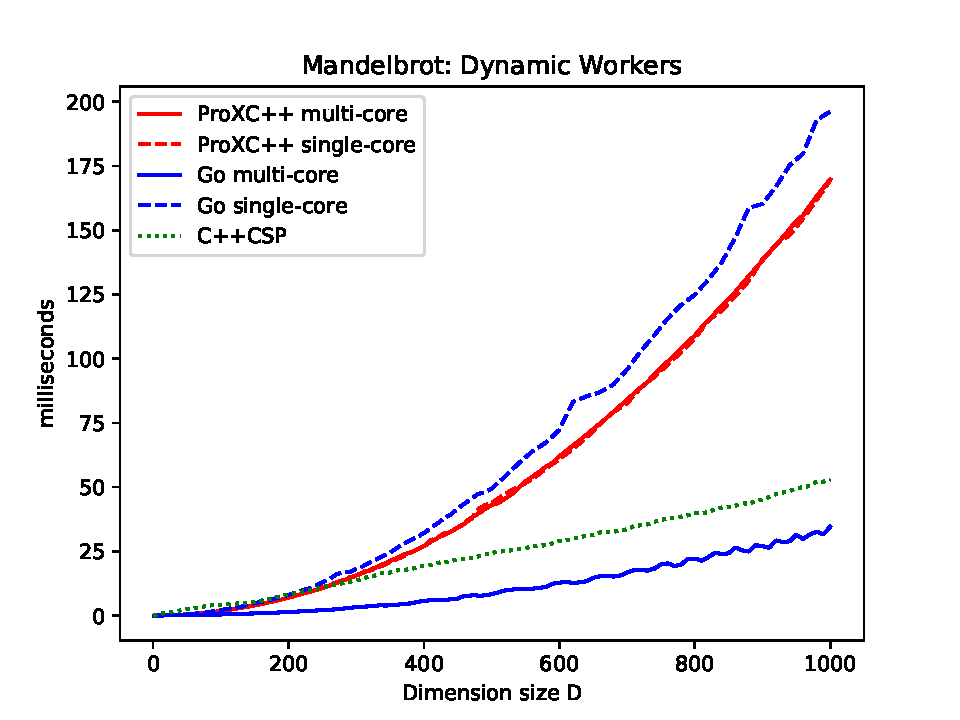
\includegraphics[width=0.9\linewidth]{fig/mandelbrot_dynamic}
    \caption{Results of concurrent Mandelbrot with dynamic number of workers.}
    \label{fig:mandelbrot_dynamic}
\end{figure}


\FloatBarrier
%%%%%%%%%%%%%%%%%%%%%%%%%%%%%%%%%%%%%%%%
\subsection{Concurrent Prime Sieve}


The last benchmark is the concurrent prime sieve, popularized by the famously elegant piece of concurrent code in Go \citep{go2017primesieve}. A prime sieve is a fast type of algorithm to find prime numbers, usually implemented as a sequential algorithm. A concurrent prime sieve is also an algorithm to find prime numbers, however daisy\hyp{}chains processes to determine whether a number is a prime or not. 

At the start of the daisy\hyp{}chain is the \textit{generator} process, which generates all numbers from $2$ and above. Along the daisy\hyp{}chain is \textit{filters} processes, where each filter represents a prime number along the number line. When the filter receives a number, the divisibility of that number is checked against the filters prime number. A non\hyp{}divisible number is passed along the daisy\hyp{}chain, while a divisible number is discarded. Given a daisy\hyp{}chain of $N$ filters, at the end of the daisy\hyp{}chain is the $N$th prime.

Note that the concurrent prime sieve algorithm is nowhere near as efficient as the sequential counterpart. The interesting merits of the concurrent prime sieve algorithm is however the total concurrent throughput. As multiple integers can be pipelined simultaneously in the daisy\hyp{}chain, it is possible to sieve multiple integers in parallel.

This benchmark test generates $N$ prime numbers, where $N=10$ to $1000$. Given a $N$, the execution time per prime number is calculated over the average running time of $10$ runs.

The results for the concurrent prime sieve test are presented in \cref{fig:concurrent_sieve}.

\begin{figure}[h!]
    \centering
    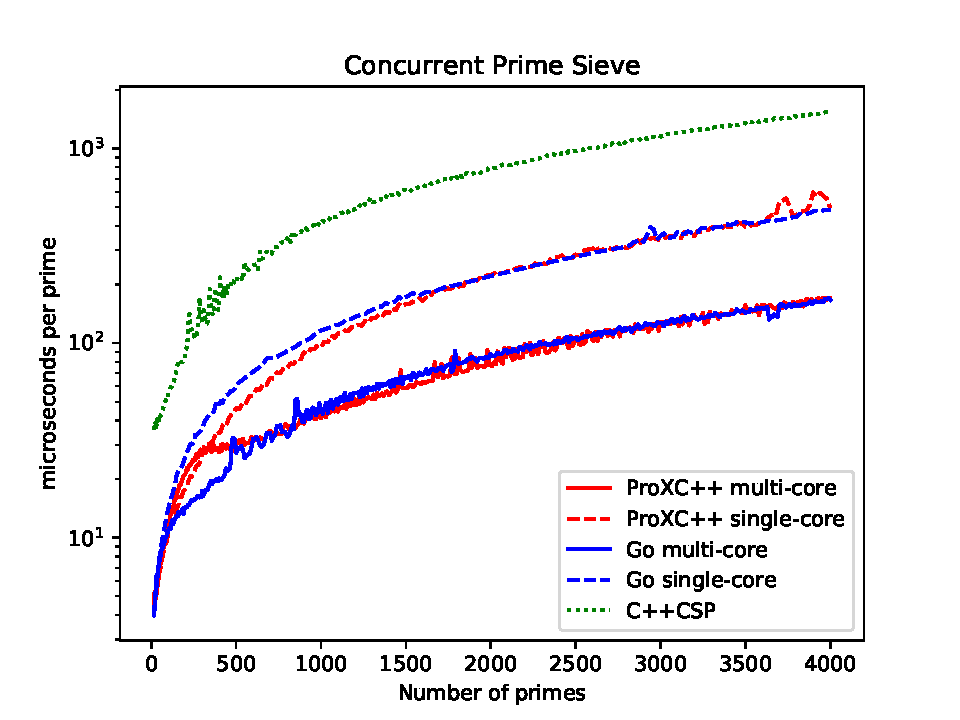
\includegraphics[width=0.9\linewidth]{fig/concurrent_sieve}
    \caption{Results of concurrent prime sieve. The Y axis has a logarithmic scaling.}
    \label{fig:concurrent_sieve}
\end{figure}


\FloatBarrier
%%%%%%%%%%%%%%%%%%%%%%%%%%%%%%%%%%%%%%%%%%%%%%%%%%%%%%%%%%%%%%%%%%%%%%%%%%%%%%%%
\section{Analysis}
\label{sec:analysis}


Starting with the extended commstime test, the results in \cref{fig:extended_commstime} shows both multicore and singlecore versions \Proxc{} and Go equals in execution time. A small exception is \Proxc{} being slightly faster than Go in the range $n\in[1;\sim{}300]$. As the chain length increases, both \Proxc{} and Go converges to a fixed execution time per chain, showing a linear increase in total execution time. 

The singlecore versions of both entries was expected to be the fastest, as extended commstime is nothing but a long sequential dependent cycle of processes. That both multicore versions matches, and sometimes surpasses, the singlecore versions is a good result. C++CSP behaves very similar to \Proxc{} and Go, however at a very much worse execution time per chain. 

The results of the hard coded Mandelbrot test in \cref{fig:mandelbrot_hardcoded} were interesting, but expected. The multicore and singlecore versions of both \Proxc{} and Go respectively increase in execution time with the same exponential trend. The singlecore version was expected to perform worst, while the multicore versions was expected to have a much better execution time. What is surprising is C++CSP being the best entry here. When thinking about it, C++CSP does have the most optimal setup here. Since each worker process in C++CSP is a kernel\hyp{}thread, each thread can run independently of each other on each core. Considering C++CSP is the best possible outcome, both multicore version of C++CSP and \Proxc{} yields a decent result.

The results of the dynamic Mandelbrot test in \cref{fig:mandelbrot_dynamic} however shows a different side. The same trends for the singlecore versions can be observed. C++CSP slightly doubles in execution time, while Go almost matches the results of the hard coded Mandelbrot test for C++CSP. The big surprise is now multicore \Proxc{} equals singlecore \Proxc{}. Further inspections of the running test processor utilization reveals the runtime system only fully utilizes a single processor core. What is happening is when the worker processes are spawned, everyone is placed on the same ready queue on the same parent scheduler. All other idle schedulers fail to effectively steal work of the one parent scheduler, resulting in only one scheduler having work to run. This test clearly highlights that \Proxc{} has issues with effectively distributing a huge number of small work across the idle schedulers.

Lastly, the results of the concurrent prime sieve test in \cref{fig:concurrent_sieve} are probably the most promising results. Fully utilizing the parallel nature in the concurrent prime sieve algorithm is very unintuitive, and heavily relies on the runtime system to detect ready work and effectively distribute said work among idle schedulers. The results show that the singlecore and multicore versions of \Proxc{} and Go both follow the same trend, where the multicore versions yields a much better result than the singlecore versions. C++CSP is a lot slower than the singlecore versions of \Proxc{} and Go, showing the lack of concurrent throughput in C++CSP. 

An interesting observation to make is between the prime range $n\in[1;\sim{}500]$ \Proxc{} is a great deal slower than Go until it suddenly drop to equal. A possible explanation is not able to effectively distribute the ready work as the processes are too short lived, sort of similar to the same issue withe the dynamic Mandelbrot test. However, over a certain limit around $\sim{}500$ processes the schedulers are able to steal the processes.

